% !TEX encoding = UTF-8
% !TEX TS-program = pdflatex
% !TEX root = ../tesi.tex

%**************************************************************
\chapter{Metodologie}
\label{cap:metodologie}
%**************************************************************

%\intro{Breve introduzione al capitolo}\\

%**************************************************************
\section{Strumenti e Tecnologie utilizzate}
Per poter eseguire il confronto tra le prestazioni di database relazionali e NoSQL è stato necessario preparare tutta una serie di strumenti utili a far funzionare i database stessi e al monitoraggio dei dati contenuti al loro interno.

\subsection{Docker}
Per poter effettuare test consistenti, evitare problemi di installazione e compartimentalizzare l'ambiente di lavoro, si è deciso di sfruttare Docker. Questo software permette di virtualizzare l'esecuzione di altri applicativi in ambienti chiusi e controllati, facilitando determinati processi di sviluppo. L'utilizzo di Docker in questo progetto lo rende più maneggevole e lineare.\\
Per sfruttare questo strumento è necessario installare l'engine di Docker che ci permette di gestire i vari container che andremo a creare.\\
Nello specifico, un container è una istanziazione di un'immagine, che a sua volta è uno snapshot del software che vogliamo "dockerizzare".\\
Docker ci permette di creare più container che funzionano parallelamente e indipendentemente gli uni dagli altri. Possono tuttavia comunicare utilizzando delle porte specificate nella fase di creazione dell'immagine.\\

\noindent Nel caso di questo progetto, docker risulta utile innanzitutto per gestire il funzionamento dei due DB (che saranno PostgreSQL e MongoDB), inserendoli entrambi in un rispettivo container.\\
Per facilitare poi i processi di comunicazione con i DB verranno utilizzati altri due container contenenti delle interfacce grafiche (rfispettivamente pgAdmin e MongoExpress).

\begin{figure}[htbp]
\begin{center}
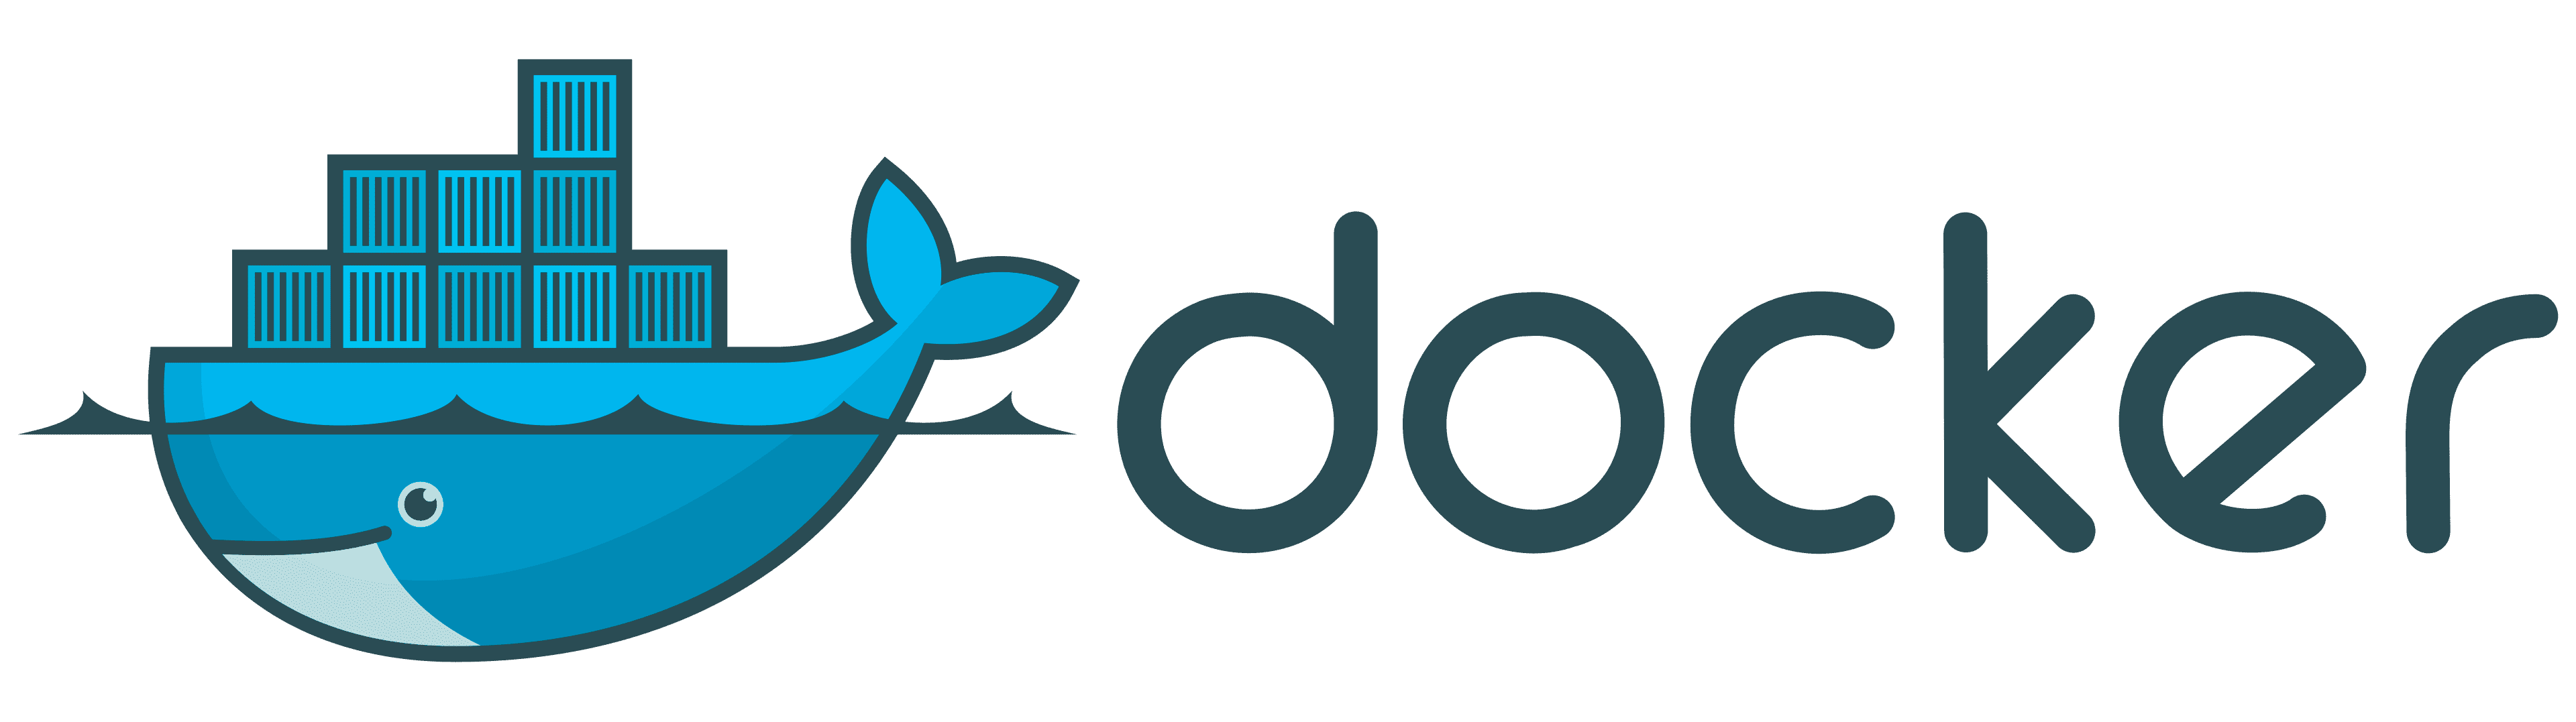
\includegraphics[height=6em]{immagini/tecnologies-logos/Docker-Logo.png}
\caption{Logo di Docker}
\end{center}
\end{figure}

\subsection{PostgreSQL e tecnologie annesse}
Dopo aver scelto Docker come ambiente in cui far girare i database, alcune altre scelte legate alle tecnologie coinvolte in questa ricerca sono state prese come conseguenza.\\
Sebbene infatti sia possibile "dockerizzare" moltissimi software, agli scopi di questa tesi è risultato più comodo partire da immagini pre-esistenti ed affidabili, disponibili sulla piattaforma ufficiale del software (hub-docker).\\
Questo ha permesso di non investre troppo tempo nella preparazione degli strumenti e di concentrare le risorse disponibili nell'effettivo confronto tra database.\\

\noindent Per tutti questi motivi si è quindi scelto di usare PostgreSQL come database relazionale da portare a confronto con MongoDB.\\
PostreSQL è un database relazionale open source molto robusto che si presta bene per rappresentare le prestazioni di un generico database di questa categoria. Esso è inoltre presente nell'hub di docker con un'immagine ufficiale, ed è quindi facile da far funzionare all'interno di un container a differenza di altri prodotti simili.\\
Sebbene PostgreSQL non sia utilizzato massivamente all'interno dell'azienda, risulta comunque molto simile alle sue controparti non open source, MSSQL e Oracle Server, che sono invece largamente uaste all'interno di Ifin e sarebbero oggetto di una potenziale migrazione qualora i risultati di questa tesi si rivelassero convincenti.\\

\noindent Vale la pena di evidenziare che a differenza delle tecnologie che ricadono sotto la sigla "NoSQL", quelle legate ai database relazionali sono molto più simili tra loro, poichè condividono appunto il paradigma relazionale che sta alla base di tutte le variazioni esistenti proposte da aziende diverse in contesti diversi.\\
In questo senso, usare PostgreSQL non è una scelta incoerente con i motivi che hanno dato alla luce questo progetto.

\begin{figure}[htbp]
\begin{center}

\includegraphics[height=7em]{immagini/tecnologies-logos/postgresql-logo.png}
\caption{Logo di PostgreSQL}
\end{center}
\end{figure}

\subsection{MongoDB e tecnologie annesse}

%**************************************************************
\section{Selezione di un ambito di confronto}

%**************************************************************
\section{Modellazione del database in MongoDB}